%# -*- coding: utf-8-unix -*-
%%==================================================
%% chapter02.tex for SJTU Master Thesis
%% based on CASthesis
%% modified by wei.jianwen@gmail.com
%% Encoding: UTF-8
%%==================================================

\chapter{过程控制系统的错误序列注入攻击}
\label{chap:FSIattack}

\section{引言}
\label{sec:intro}

过程控制系统作为国家关键基础设施的基本组成部分已经广泛应用于工业和物联网系统中。正因为它们在现代工业社会中的关键作用,使得它们成为怀有恶意目的的攻击者的感染和侵袭的目标。传统的安全保护主要是通过多层网络防火墙和成熟的的病毒防御软件阻止网络攻击入侵工业网络。然而考虑到网络和复杂的硬件系统实施,这些方法不能完全保护网络和硬件平台免受不断变异的威胁侵入,例如Stuxnet病毒侵入人机界面(HMI)服务器并上传恶意代码到可编程逻辑控制器PLC使其损坏制造核原料的离心机。考虑到HMI服务器通常安放在在受良好保护的工业控制网络中,所以对其实施攻击是非常困难的。
本章我们提出的错误序列注入(FSI)攻击,可以通过感染和篡改PLC的输入信号迫使其执行误操作和破坏控制系统的关键设备。因为PLC的输入仅仅来自假设被FSI攻击注入的远程传感器,所以在不需要渗透到防御坚固的控制网络并执行恶意代码上传的情况下便可以对系统实施有目的性攻击。值得注意的是我们构造的攻击可以避开现有的系统故障检测机制,并利用其容错率漏洞来构造基于离散时间模型的FSI攻击。

\section{攻击模型概述}
\label{sec:formulation}

考虑到图1描述的威胁模型,攻击者只需要侵入并控制遍布在远程的信号采集传感器。从过去的假数据注入攻击研究[5],[9],[19],[20],[30]中我们知道大部分工业控制系统包括电力系统的远程传感器如相量测量单元在实践中受到的保护较少并且分布在全国各地,因此与控制网络内的服务器相比更容易访问和侵入。我们假设攻击者知道高级基础设施配置,即连接到PLC传感器和执行器的输入输出的变量映射关系,这样攻击者不必渗透到控制网络中FSI攻击仍然可以成功。即使HMI服务器没有泄密而且攻击者也没有获得在PLC设备上上传恶意控制器程序的权限,我们构造的错误序列攻击只需要注入并控制向PLC发送测量信号的传感器便可以对控制系统造成不可逆的破坏。

\begin{figure}[!htb]
  \centering
  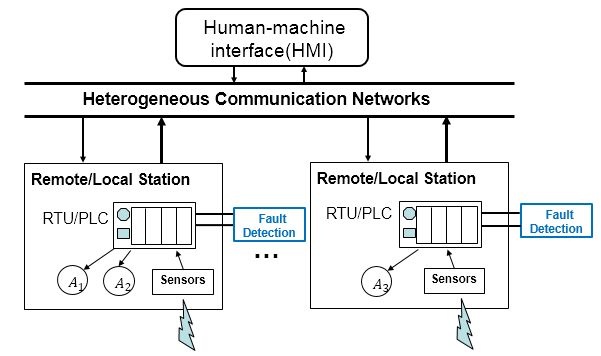
\includegraphics[scale=0.29]{att/threatModel1.png}
  \caption{FSI攻击威胁模型}
  \label{fig1}
\end{figure}

然而困难是如何在现有控制系统中部署的成熟故障检测的情况下构建攻击使PLC执行误动作。FSI攻击的主要任务之一是分析并且绕开故障检测机制。通常来看用辨识精度不高的系统模型来检测随机性的故障能够得到很高的准确度,我们通过这一特性反向构造错误序列并且注入到受控制的远程传感器则可以达到使故障检测失效的目的。图\ref {fig2}显示了攻击是如何构造的。我们假设对手可以访问在PLC控制器和物理设备之间交换的信号或堆栈数据。然后利用输入和输出向量数据库,我们辨识出与故障检测的建模方法类似的无故障的离散事件模型。最后,我们搜索所有的不可被故障机制检测的虚假序列的集合,并且获得适当长度的恶意序列对受控制的传感器采集的输入信号进行篡改。

\begin{figure}[!htb]
  \centering
  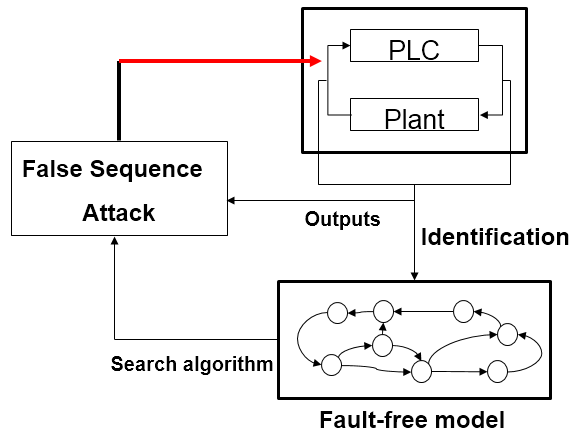
\includegraphics[scale=0.3]{att/ASC2.png}
  \caption{FSI攻击构造示意图}
  \label{fig2}
\end{figure}

\section{系统建模和攻击构造}
\label{sec:model}

我们需要一个形式化的描述来辨识特征值为$m$的系统模型$ \textbf{BEH}_{Ident}^m $和观测信号模型\( \textbf{BEH}_{Obs}^m \),从形式化模型定量生成特征值大于$m$特征向量。辨识的目标是使得在给定便是参数$k$的条件下特征值超出$k$的特征向量数目达到最小,理想情况是$ \textbf{BEH}_{Ident}^m $与$\textbf{BEH}_{Obs}^m $相等。最后我们在辨识得到的系统模型和观测信号模型基础上搜索FSI攻击序列。

\subsection{信号采集和观测特性定义}

我们通过在PLC控制器获取信号之后以固定时间间隔读取信号来采样数据\cite {roth2012}。图\ref {fig3}显示了从PLC采样$I/O$向量序列的最常用的方法,通过OPC通信模式收集在服务端接收到的$I/O$数据形成标识数据库。

\begin{figure}[!htb]
  \centering
  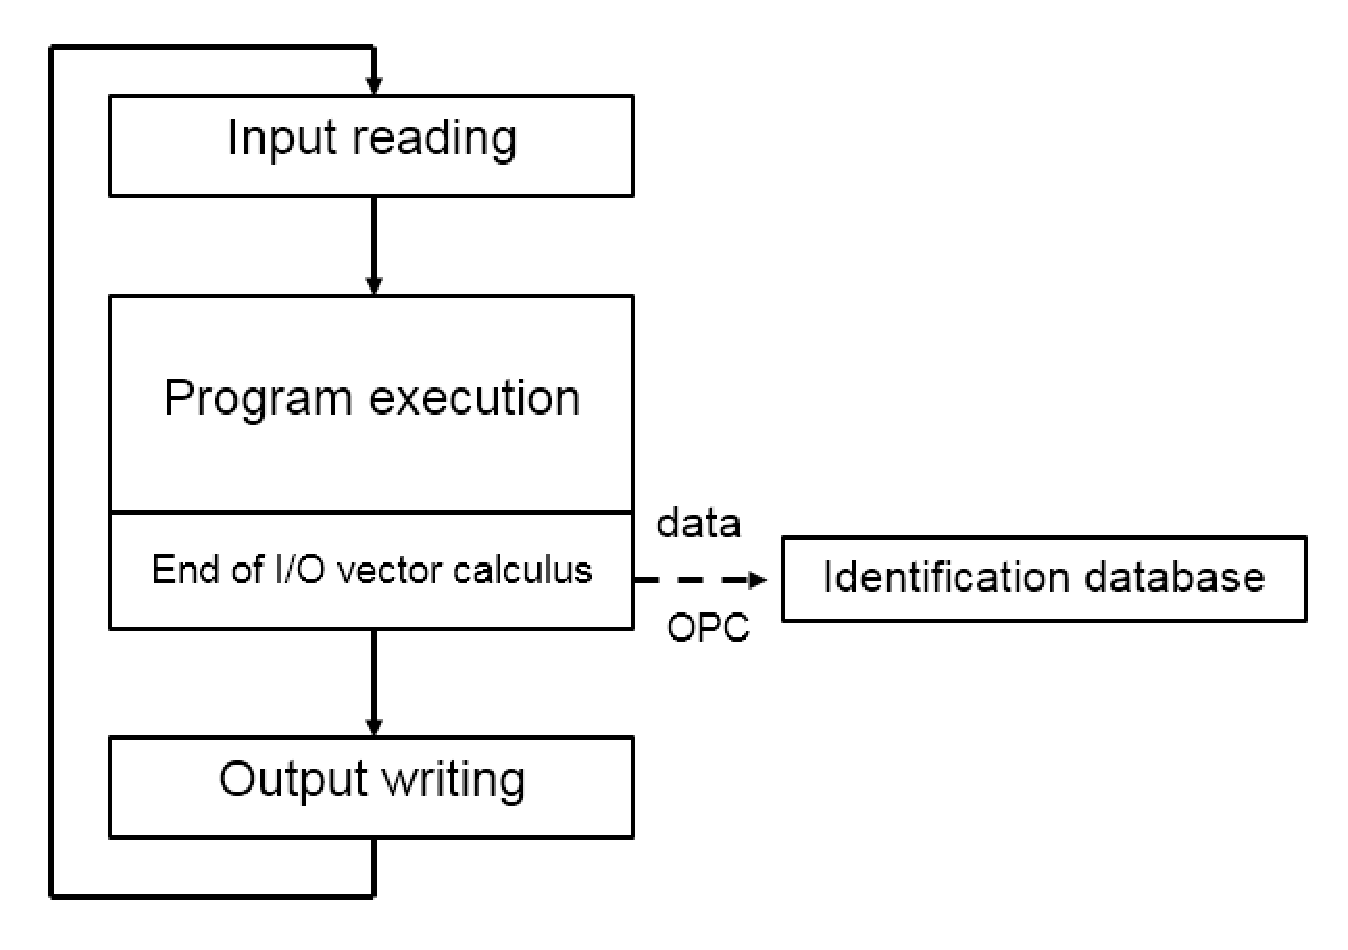
\includegraphics[scale=0.3]{att/database2.eps}
  \caption{对PLC采样数据示意图}
  \label{fig3}
\end{figure}

在实现数据收集之后,我们需要定义观察到的输入/输出($I/O$)序列、采样数据的语义和词义。 首先我们引入以下定义,

\textbf{定义1:} \( r \)个输入和$ s $ 个输出的采样数据的观测$I/O$序列集合定义为:

\begin{equation} 
\Sigma = (\gamma_1,...,\gamma_p) 
\end{equation} 这里 $\gamma_i = (u_i(1),u_i(2),...,u_i(|u_i|))$, $ u_i(j) $ 是第$i$个$I/O$向量$u$的第$j$个输出,其中$ u = (I_1,...,I_r,O_1,...,O_s) = (IO_1,...IO_m) $ 且 $ m=r+s $.

我们假设对于$ \forall $两个连续的$I/O$向量$ u(t)\ neq u(t + 1)$ 成立
当且仅当至少一个$I/O$向量分量改变且$I/O$向量是新生成的。

\textbf{定义2:} 观测到的采样数据词义集合表示和语义集合表示: 观测的词义可以用$I/O$序列长度为$q$的观测向量集合描述 
\[
L_{Obs}^q = \bigcup_{\gamma_i \in \Sigma} \Big(\bigcup_{t=1}^{|\gamma_i|-q+1} (u_i(t),u_i(t+1),...,u_i(t+q-1))\Big) 
\]

有了词义的形式化表示后,我们定义长度为$n$的采样数据的语义的表示:
\begin{equation}
 \textbf{BHE}_{Obs}^n = \bigcup_{i=1}^n L_{Obs}^i 
\end{equation}

\subsection{模型辨识}

\subsubsection{模型选择}

模型辨识的目的是确保辨识的任意长度为$ m $的语义表示$ \textbf {BEH}_{Ident}^m $等于观测到的任意长度为$ m $的语义表示  \( \textbf{BEH}_{Obs}^m \),其中$ m $可以是任何正整数。 简而言之,所辨识的模型在精度足够高的情况下能够完美复现基于PLC的过程控制系统。考虑到过程控制系统通常是可编程的控制器和物理设备的耦合系统,可编程的控制器可以被认为是确定性的,而物理设备通常被认为是非确定性的。因此,物理设备和控制器的耦合系统一定是非确定性的。因此,我们提出了适合于辨识过程控制系统的非确定性自发输出自动机(NDAAO)\parencite{klein2005}。

\textbf{定义3:} NDAAO是由5元组函数表示: \[ NDAAO=(X,\Omega,\textit{f}_{nd},\lambda,x_0) \] with\
\begin{itemize}
  \item $ X={x_0,...,x_{|x|-1}} $ 是有限状态集
  \item $ \Omega={\omega_1,...,\omega_{|\omega|}} $ 是有限输出变量集
  \item $ \textit{f}_{nd}: X\rightarrow 2^X $ 是非确定性转移函数
  \item $ \lambda: X\rightarrow \Omega $ 是状态对应的输出函数
  \item $x_0$ 是初始状态
\end{itemize}

NDAAO可以由图$G=(V,E)$的形式表示,图$G$的定点集是NDAAO所有的状态集,有向边集是由非确定性转移函数$f_{nd}$组成,即\[ E(G)=\big\{(x_i,x_j)\in X\times X: x_j\in f_{nd}(x_i)\big\} \],每个节点对应一个状态并包含状态对应的输出,图~\ref{fig4}通过一个简单的例子来展示图形化的NDAAO模型。

\begin{figure}[!htb]
  \centering
  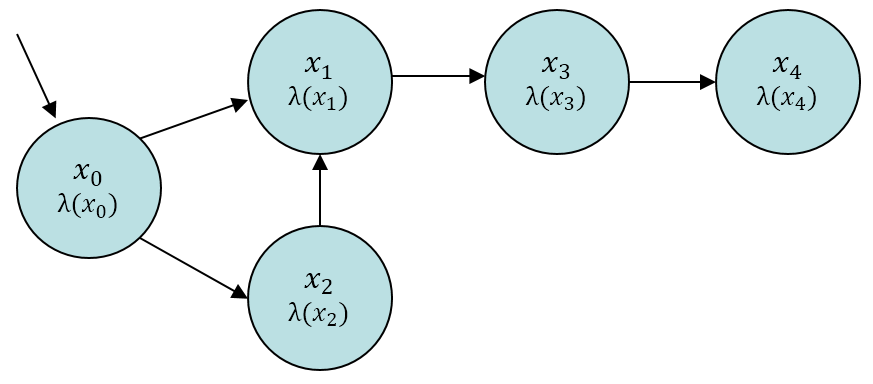
\includegraphics[scale=0.18]{att/ndaao_example.png}
  \caption{NDAAO图形表示}
  \label{fig4}
\end{figure}

\textbf{定义4:} NDAAO的词义和语义表示: 由开始状态为$x_i$NDAAO生成的长度为$n$词语集合表示为
\begin{equation} 
W_{x_i}^{n}=\left\{\begin{split} &w\in \Omega^n~|~ w=\big( \lambda(x(1),...,\lambda(x(n))) \big):\\ 
&[\exists \big(x(1),...,x(n)\big): x(1)=x_i\in X,~and\\
&\forall\;1\leq t\leq n-1, x(t+1)\in f_{nd}(x(t))] \end{split} \right\} 
\end{equation} 然后由词语组成的长度为$n$词组集合表示
\begin{equation} 
W^n(NDAAO)=\bigcup_{x_i\in X} W_{x_i}^{n} 
\end{equation} 有了词组集合,我们可以获得NDAAO的长度为$n$语义集合表示
\begin{equation} 
\textbf{BEH}_{Ident}^n=\bigcup_{p=1}^n W^{p}(NDAAO) 
\end{equation}

\textbf{定义5:}辨识事件向量$\varepsilon(j)$是NDAAO中相邻两个辨识输出向量$\omega(j)$ 和 $\omega(j+1)$ 的变化量,用公式表示为 $\varepsilon=\omega(j+1)-\omega(j)$. 输入事件向量 $I(\varepsilon(j))$ 是相邻两个辨识输入向量 $I(j)$ 和 $I(j+1)$的变化量,同理输出事件向量$O(\varepsilon(j))$也有相似的定义. 具体的公式表示为:
\begin{equation} 
\varepsilon(j)=\bigcup_{l=1}^m \begin{cases}
I_l\_1~or~O_l\_1,~if~ I_l(j+1)-I_l(j)=1\\
I_l\_0~or~O_l\_0,~if~ I_l(j+1)-I_l(j)=-1\\
\epsilon,~if~ I_l(j+1)-I_l(j)=0
\end{cases} 
\end{equation}

考虑包含两个输入和一个输出的$I/O$向量序列$\gamma$,我们得到 \[\gamma=(A,B,C)=( \begin{bmatrix}
0\\1\\0
\end{bmatrix},\begin{bmatrix}
1\\1\\0
\end{bmatrix},\begin{bmatrix}
1\\0\\1
\end{bmatrix})\]

该序列可以简化表示成 $A\xrightarrow{I_1\_1}B\xrightarrow{I_2\_0,O_1\_1}C\cong A\xrightarrow{I_1\_1,I_2\_0,O_1\_1}C$

\subsubsection{辨识算法}

本节我们提出了一个辨识算法用来生成上一节中所描述的NDAAO模型。我们定义辨识参数$ k $用于确定用于生成新状态的$I/O$向量序列的长度。如果生成的NDAAO模型的长度为$ k $的语义集合正好与观测时采样数据产生的长度为$k$的语义集合一致的话,这样的NDAAO模型被称为$ k $完全可观测的。

NDAAO的构造主要分为三个步骤。首先,我们将观察到的序列转换为一组长度为$ k $的词组序列并在每组的第一个状态前创建一组长度为$ k-1 $ 伪状态以确保与其他词语一致。算法1的第一部分表示了观测序列的转换过程。然后我们开始执行NDAAO辨识操作, 将NDAAO的状态集与长度为$ k $的词组集相关联,并且转移函数由长度为$ k+1 $的词语表示。算法1的第二部分表示了NDAAO的辨识过程​​。最后,我们合并等效状态来对状态空间进行降维,对于任意两个不同的状态$ x_i $和$ x_j $,如果它们相关联的输出相同并且它们具有相同的后继状态集,则我们可以将这两个状态合并到一个状态。我们通过从NDAAO的状态集和转移函数绘制状态转移图来使模型可视化。具体过程如算法1的第三部分所示。

\renewcommand{\algorithmicrequire}{\textbf{输入:}}
\renewcommand{\algorithmicensure}{\textbf{输出:}}
\begin{algorithm}[h]
  \caption{Construction of the NDAAO}
  \begin{algorithmic}[1]
    \REQUIRE %算法的输入参数:Input  
    观测的$I/O$序列(采样数据) $\varSigma$ 和辨识参数 $k$ \\  
    
    \ENSURE %算法的输出:Output  
    NDAAO模型和状态转移图 $G=(V,E)$;  \\
    // \textbf{第一部分:}观测序列的转换过程
    \FOR{each $\gamma_i \in \varSigma$}
      \IF {$u_i(1)\neq u_i(|\gamma_i|)$}
          \STATE  从$\varSigma$删除$\gamma_i$;\
          \STATE Return;\
        \ELSE
        \STATE $\alpha_i(t)=\begin{cases}
        u_i(1),\quad for ~~ 1\leq t\leq k-1\\
        u_i(t-k+1),\quad for ~~ k \leq t \leq k+|\gamma_i|-1
        \end{cases}$\
        \FOR {$m=1~~to~~|\gamma_i|$}
        \STATE $w_i(m)=(\alpha_i(m),...,\alpha_i(m+k-1))$;
        \ENDFOR
        \STATE $\gamma_i^k=(w_i(1),...,w_i(|\gamma_i|))$;
        \ENDIF
    \ENDFOR
    \STATE $\varSigma^k=\bigcup\limits_{i=1}^{|\varSigma|}  \gamma_i^k$;\\
    // \textbf{第二部分:}NDAAO的辨识过程​​
    \STATE 初始化状态集 $X=\emptyset$, 转移函数 $f_{nd}(x_0)=\emptyset$, 输出 $\Omega=\emptyset$, 初值状态 $x_0=\varSigma^k[0][0]$, 节点集 $N=\emptyset$ 和边集 $E=\emptyset$;
    \FORALL {$\xi$ such that $\xi \in \varSigma^k$} 
      \FORALL {$\eta$ such that $\eta \in \xi$}
      \STATE $X\leftarrow X\cup \xi$; 
      \STATE $\Omega \leftarrow\ \Omega \cup \eta(|\eta|)$;
      \ENDFOR
    \ENDFOR
    \FORALL {$\delta$ such that $\delta \in \varSigma^{k+1}$} 
      \FORALL {$\psi$ such that $\psi \in \delta$}
      \STATE $x \leftarrow \psi[1-k]$;
      \STATE $f_{nd}(x)=\psi[k-|\psi|]$;  
      \ENDFOR
    \ENDFOR\\
    //\textbf{第三部分:}状态空间降维和图形化表示
    \FORALL {$x_i,x_j$ such that $x_i,x_j \in X and i\neq j$} 
      \IF {$\lambda(x_i)=\lambda(x_j)$ 和 $f_{nd}(x_i)=f_{nd}(x_j)$}
        \STATE 合并 $x_i$ 和 $x_j$, 从$X$中删除 $x_i(x_j)$ 并且用$f_{nd}(x_{pre})=x_j(x_i)$替换$f_{nd}(x)=x_i(x_j)$, 这里$x_{pre}$是$x_i(x_j)$的前继;  
      \ENDIF
    \ENDFOR
    \STATE $V\leftarrow\ V\cup X$; 
    \STATE $E \leftarrow E\cup (x,f_{nd}(x))$;
    \STATE 对$G(V,E)$画图;
  \end{algorithmic}
\end{algorithm}

\section{实验仿真}
\label{sec:simulation}

\section{本章小结}
\label{sec:insertimage}

